\documentclass[10pt,a4paper]{book}
\usepackage[utf8]{inputenc}
\usepackage[spanish]{babel}
\usepackage{amsmath}
\usepackage{amsfonts}
\usepackage{amssymb}
\usepackage{makeidx}
\usepackage{graphicx}
\usepackage{fourier}
\usepackage{color}
\usepackage{fancyvrb}
\usepackage{hyperref}
\author{Maqueavelo Hidrovo, José Jácome, Erik Quijije}
\title{Proyecto II}
%Comando para hacer un rectangulo en una palabra
\newcommand{\HRule}{\rule{\linewidth}{0.5mm}}

\begin{document}
\begin{titlepage}
\begin{center}

\includegraphics[scale=1]{espe.jpg}\\ 
\vfill
\textsc{\LARGE UNIVERSIDAD DE LAS FUERZAS ARMADAS ESPE}\\[1.5cm] 
\textsc{\Large Proyecto de Matemática Superior}\\[0.5cm] 
% Title
\HRule \\[0.4cm]
{ \huge \bfseries Desarrollo de varias ondas de audio a través de una síntesis de Fourier.
 \\[0.4cm] }

\HRule \\[1.5cm]
\textsc{\Large AUTORES}\\[0.5cm]
\emph{\Large \begin{itemize}
\item Hidrovo Andrés	
\item Jácome José
\item Quijije Erik
\end{itemize}}


\vfill

% Bottom of the page
{\large \today}

\end{center}
\end{titlepage}
\tableofcontents % indice de contenidos
\addcontentsline{toc}{chapter}{Lista de figuras}
\cleardoublepage
\pagenumbering{arabic}


\section{Tema}

Desarrollo de varias ondas de audio a través de una síntesis de Fourier.\\

\section{Objetivo General}

Generar varias ondas de audio para desarrollar una aplicación con la Serie de Fourier. \\

\section{Objetivos Específicos}

Aproximar una onda de audio mediante un análisis por la serie de Fourier.\\
Generar varias ondas de audio de diferente forma y amplitud.\\
Usar un circuito amplificador para aumentar la amplitud de la onda.\\

\section{Marco Teórico}

Fourier  es una técnica matemática, desarrollada hace más de siglo y medio por Joseph Fourier y publicada en su libro \textit{Théorie analitique de la chaleur}, y que da cuenta de la complejidad de los sonidos, más allá de las características de intensidad-tono-timbre.\\
\subsection{Espectro Sonoro de un Sonido Complejo}

El análisis a la Fourier de un sonido lo descompone en todas y cada una de las frecuencias que lo forman, y le asigna a cada frecuencia una intensidad o amplitud específica. Al conjunto de frecuencias amplitudes se le llama el espectro del sonido analizado.
En un sonido nuestra sensación de tono que no está determinada únicamente por la "frecuencia" del sonido, cuando éste es complejo, ya que, sencillamente, un sonido complejo no tiene una sola frecuencia, y ni siquiera bastan para definirlo sus armónicos principales. La sensación de "un" sonido es el resultado de toda una serie de ondulaciones de distintas frecuencias, cuyas importancias relativas cambian rápidamente con el tiempo.\\

\begin{center}
	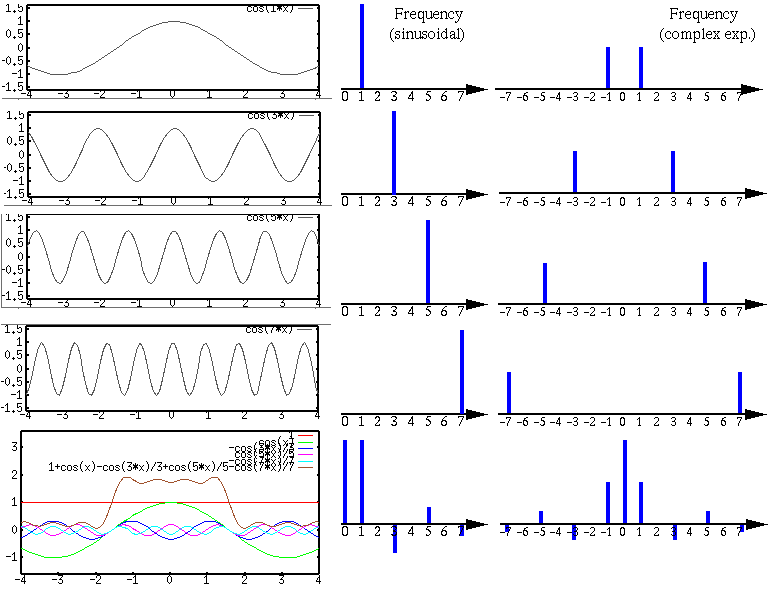
\includegraphics[scale=0.45]{AudioFourier.png}\\
\end{center}

Cualquier forma de onda, a condición de que sea periódica (se repita siempre igual) se puede descomponer en una serie más o menos larga (quizás infinita) de ondas puras (senoidales) llamadas armónicos. Estos armónicos son tales que su combinación o mezcla dan lugar de nuevo al sonido original, y sus frecuencias son múltiplos enteros de la del sonido fundamental.\\

\textbf{Proposicion 1}\\
%Para todo $n,p,e \epsilon 0 \cup N$ se cumple que: \\

\begin{center}
	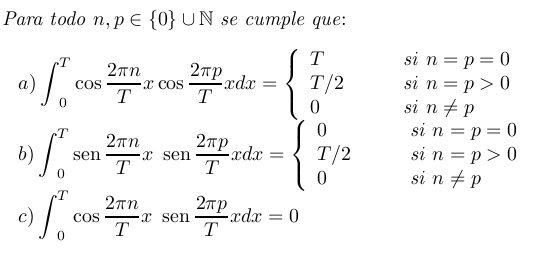
\includegraphics[scale=0.45]{AudioFourier2.png}
	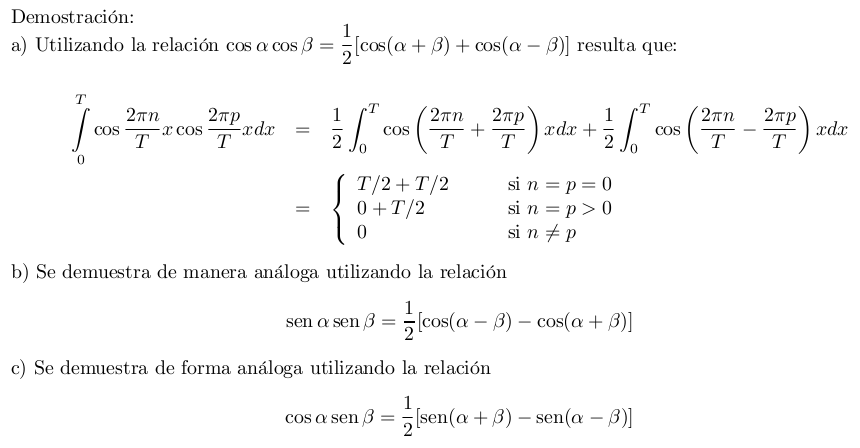
\includegraphics[scale=0.45]{AudioFourier3.png}
\end{center}

\textbf{Proposicion 2}\\
Si  $g  : R \rightarrow R$  es una función T-periódica e integrable en un intervalo de longitud T,    entonces se verifica:\\

\begin{center}
	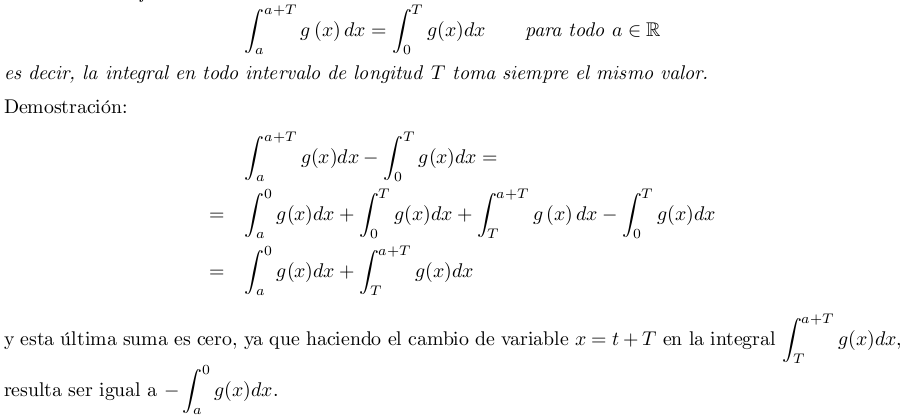
\includegraphics[scale=0.45]{AudioFourier4.png}
\end{center}

\textbf{Proposicion 3}\\
Si $f:[-a,a] \\rightarrow R  $ es integrable, se puede asegurar que: \\

\begin{center}
	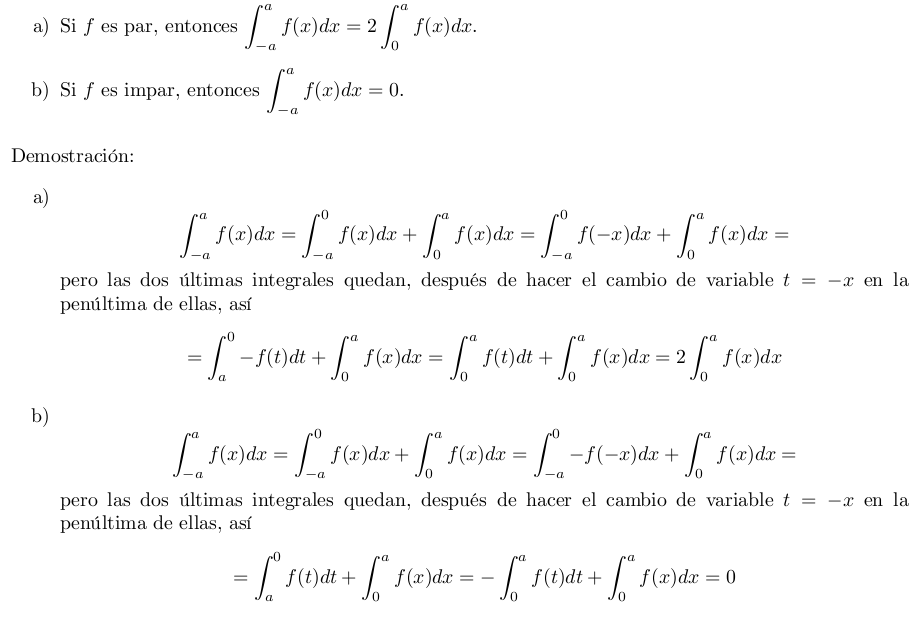
\includegraphics[scale=0.45]{AudioFourier5.png}
\end{center}

\subsection{Programación en Scilab}

\begin{verbatim}
clc 
clear 
printf('\n\nProyecto de matematicas superior/n /n') 
printf('\n\nIntegrantes:') 
printf('\n\nJose Jacome\t Maqueavelo Hidrovo\t Erik Quijije\n\n') 

sample_rate=input('ingrese el periodo'); 
inicio=input('ingrese el rango de inicio') 
final=input('ingrese el rango a terminar') 
t = inicio:1/sample_rate:final; 

N=size(t,'*'); //number of samples 
r=input('ingrese la funcion f(t)') 
//s=sin(2*%pi*50*t)+sin(2*%pi*70*t+%pi/4)+grand(1,N,'nor',0,1); 
 s=r+grand(1,N,'nor',0,1); 
y=fft(s); 

//s is real so the fft response is conjugate symmetric and we retain only the first N/2 points 
f=sample_rate*(0:(N/2))/N; //associated frequency vector 
n=size(f,'*') 
clf() 
plot(f,abs(y(1:n)))
\end{verbatim}

\subsection{Equipo usado para la reproducir el sonido: Raspberry Pi}

Un Raspberry Pi es una computadora de bajo costo, del tamaño de una  tarjeta de crédito que se conecta a un monitor de ordenador o un televisor, y utiliza un teclado y un ratón estándar. Es un dispositivo pequeño que permite a las personas de todas las edades a explorar la computación, y para aprender a programar en lenguajes como Python y Scratch. Es capaz de hacer todo lo que espera que una computadora haga, desde navegar por Internet y reproducción de vídeo de alta definición, hacer hojas de cálculo, procesadores de texto, y jugar juegos.\\

Lo que es más, el Raspberry Pi tiene la capacidad de interactuar con el mundo exterior, y se ha utilizado en una amplia gama de proyectos  digitales, desde las máquinas de música y detectores de sonido hasta estaciones meteorológicas y  pajareras con cámaras infrarrojas. Queremos ver la Raspberry Pi siendo utilizado por los niños de todo el mundo para aprender a programar y entender cómo funcionan las computadoras.\\

\begin{center}
	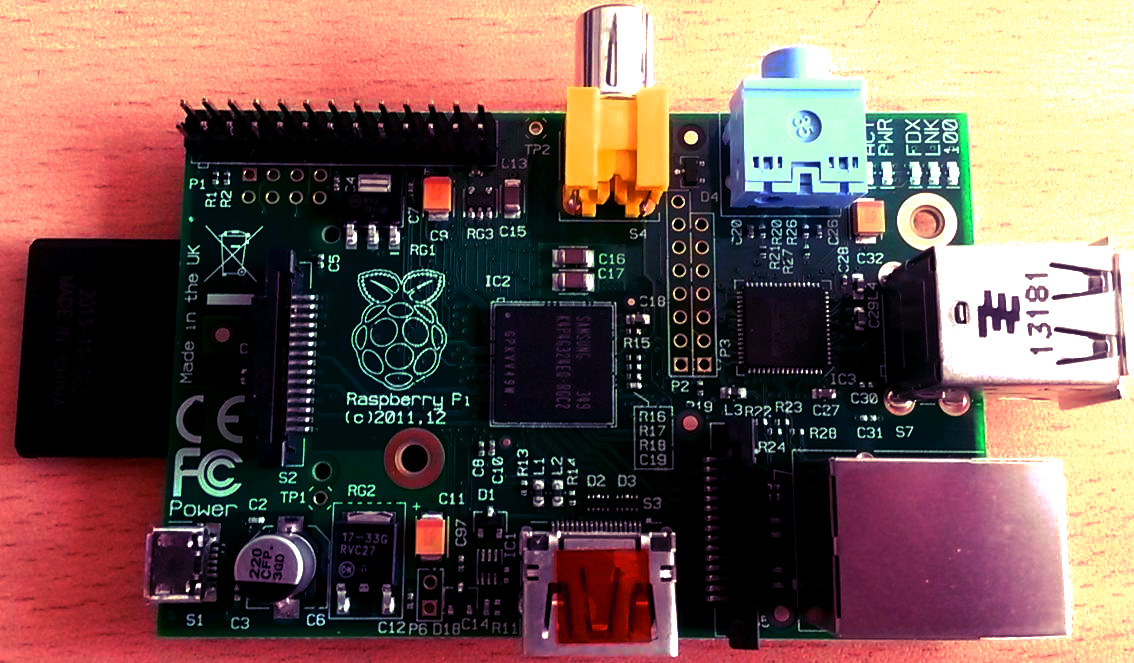
\includegraphics[scale=0.35]{raspberry.jpg}
\end{center}

\subsection{Puertos GPIO}

GPIO (General Purpose Input/Output, Entrada/Salida de Propósito General) es un pin genérico en un chip, cuyo comportamiento (incluyendo si es un pin de entrada o salida) se puede controlar (programar) por el usuario en tiempo de ejecución.\\

Los pines GPIO no tienen ningún propósito especial definido, y no se utilizan de forma predeterminada. La idea es que a veces, el para el diseño de un sistema completo que utiliza el chip podría ser útil contar con un puñado de líneas digitales de control adicionales, y tenerlas a disposición ahorra el tiempo de tener que organizar circuitos adicionales para proporcionarlos. Por ejemplo, los chips Realtek ALC260 (códec de audio) tienen 8 pines GPIO, que quedan sin utilizar de forma predeterminada. Algunos integradores de sistemas (Acer Inc. laptops) que emplea el ALC260 utilizan la primera GPIO (GPIO0) para encender el amplificador utilizado para los altavoces internos y el conector de auriculares del ordenador portátil.\\

\subsection{Codigo para generar una onda de sonido}

El siguiente código puede ser ejecutado sobre un Raspberry Pi gracias al Lenguaje de Programación Python y la librería Wiringpi2
\begin{verbatim}
import sys
import time
import wiringpi2

io = wiringpi2.GPIO(wiringpi2.GPIO.WPI_MODE_PINS)

wiringpi2.softToneCreate(7)

wiringpi2.softToneWrite(7,int(sys.argv[1]))
time.sleep(float(sys.argv[2]))
\end{verbatim}



\section{Conclusiones}

\begin{itemize}

\item El análisis espectral de señales continuas y no periódicas se puede llevar a cabo usando Fourier, con aproximación de una o de varias ondas que forman la onda la onda de sonido.
\item El sonido es una onda periódica en el tiempo que se puede ajustar fácilmente a una serie de Fourier, tomando en cuenta se amplitud modulo, entre otras, ya que estas le  dan las características y comportamiento de las ondas espectrales. 
\item El circuito amplificador permitió reproducir y apreciar la forma sonora de las ondas espectrales de sonido por medios auditivos, pudiendo constatar la onda producida.

\end{itemize}

\section{Recomendaciones}

\begin{enumerate}
\item Realizar los cálculos en un software matemático y el diseño en un programa que permita simular correctamente la onda de sonido con los diferentes parámetros asignados
\item Realizar la simulación del análisis por medio de equipos auditivos y observar de forma gráfica el comportamiento de estas.
\item Tener el equipo necesario para poder llevar a cabo todas las tareas de análisis, ya que al tener falencias no se podrá llegar a comprender de forma clara el trabajo realizado.

\end{enumerate}

\section{Bibliografía}

\begin{enumerate}
\item “Graficador de serie de Fourier”, http://mygnet.net/codigos/matlab/graficacion, Consultado en Junio del 2014.
\item “Señales y análisis de Fourier”, http://www.slideshare.net/psyrcd/sa-fourier-con-matlab , Consultado en diciembre del 2013.
\item “Series de Fourier”, Aplicación de las matemáticas, http://personal.us.es/niejimjim/tema07.pdf , Consultado en Junio del 2014
\end{enumerate}

\end{document}